%!TEX root = ../physical-olympics-2.tex
\chapter{液体与固体的性质}

在讲解热力学基本规律的过程中,\,我们已经对气体,\,尤其是理想气体这样的热力学体系有了一定的了解.\,但是对于与我们的生活息息相关的\emph{液体}(liquid)与\emph{固体}(solid)两种\emph{凝聚态}(condensed matter)我们还知之甚少.\,在此稍作一步展开介绍.

\section{固体晶格论}


\begin{wrapfigure}[8]{o}[-10pt]{7cm}
\centering
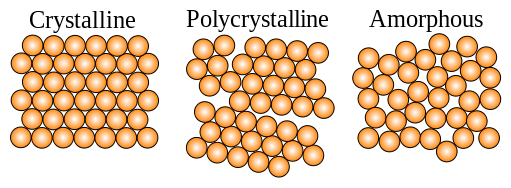
\includegraphics[width=7cm]{image/5-3-2.png}
\caption{单晶体,\,多晶体与无定形体}\label{fig:3crystal}
\end{wrapfigure}
固体在此处实际上特指\emph{晶体}(crystal).\,晶体应具有\emph{长程序}(long-ranged order),\,也就是说组成的晶体的原子,\,分子,\,或者离子应体现出大范围的空间周期性.\,如图\ref{fig:3crystal}所示,\,一整块物质如果完全由严格的周期性结构组成,\,那么一般其表面也是规则的几何形状,\,称作\emph{单晶体}(single crystal).\,但是大量的晶体内部是充满着\emph{缺陷}(defect)的,\,无论是原子的\emph{缺失}(vacancy)还是\emph{填隙}(interstitial),\,还是更复杂的面缺陷与体缺陷,\,都会使得晶体的不同区域变得孤立起来,\,常见的金属,\,冰,\,陶土,\,岩石都是由大量可视作晶体的晶粒拼接而成,\,在物理性质上丧失了单晶体所具有的的各向异性而成为\emph{多晶体}(polycrystal).\,最后还有丧失了长程序的\emph{无定形体}(amorphous solid),\,比如玻璃,\,蜡,\,塑料等,\,它们都不是晶体,\,但一般仍认为是固体.

固体的结合方式在极大程度上决定了其热学性质,\,而固体的结合又在很大程度上依赖于其外层的电子在量子统计规律下的诸多行为.\,根据最后的结果我们可以粗浅地分类:
\begin{figure}[H]
\centering
\begin{tabular}{c|c}
\hline
晶体类型			&		结合方式\\ \hline\hline
原子晶体			& 局域在原子间的共用价电子对与原子实之间的相互吸引 \\ \hline
离子晶体 		& 一种原子的电子几乎完全被另一种原子剥夺形成离子,\,两种离子相互吸引 \\ \hline
金属晶体			& 非局域的共享电子们与原子实们之间的相互吸引 \\ \hline
分子晶体 		& 分子与分子之间十分微弱的氢键,\,范氏相互吸引,\,还包含电偶极矩磁偶极矩相互作用 \\ \hline
\end{tabular}
\end{figure}


在某些较为简单的情形下,\,我们会认为固体可以拆解为两个体系,\,一是由\emph{原子实}(atomic core)构成的\emph{点阵}(lattice),\,一是参与原子间相互作用的所有\emph{价电子}(valance electron)构成的\emph{电子气}(electron gas).\,后者是那么地轻盈,\,但是却带有与原子实等量反号的电荷,\,这一点造成了如下的局面:\,体系的动能几乎由具有绝大多数质量的点阵承担\footnote{其实这也是个量子效应,\,详见下一章.};\,而势能也由点阵的位置与变形来计算,\,对于电子的分布,\,总是遵循泡利不相容原理和最小势能原理,\,故可由点阵位置计算.\,这种\emph{平均场论}(mean field theory)的思想使我们写出体系的总能量来:
\[E=T(\bs{v}_{i,g})+V(\bs{r}_{i,g})\quad ,\quad i=1,2\cdots n\;;\;g\in G\]

\begin{wrapfigure}[10]{o}[-10pt]{6cm}
\centering
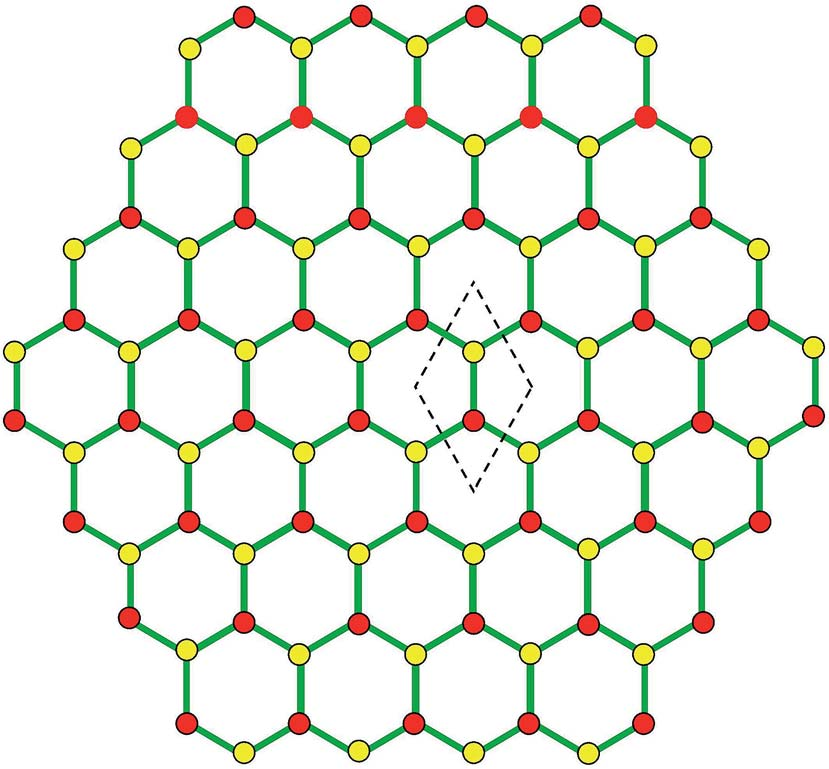
\includegraphics[width=6cm]{image/5-3-3.png}
\caption{石墨烯的结构}\label{fig:graphene}
\end{wrapfigure}
式中$G$表示所有\emph{原胞}(unit cell)的集合,\,将一个原胞按照$G$的方式平移便得到了整个晶体,\,称作\emph{布拉伐格子}(Bravais lattice).\,而每一个原胞都是全同的,\,内含$1,2\cdots n$号原子.\,以\emph{石墨烯}(graphene)为例,\,\emph{石墨}(graphite)实际上即由一层一层的石墨烯通过范德瓦尔斯力吸引而形成.\,每一层可以认为是一种平面型的晶体.\,其原胞由两个并不具有平移等价性的原子构成.\,原胞形状为菱形,\,故可以在平面上按密铺,\,


\begin{itemize}
	\item 晶体分为原子晶体,\,离子晶体,\,金属晶体,\,分子晶体...
	\item 晶格为晶体带来摩尔热容$C=3R$,\,此即\emph{杜隆-裴替定律}(Dulong-Petit law)
	\item 晶格为晶体带来热膨胀.\,$l=l_0(1+\alpha t)$.\,$\alpha$为线膨胀系数.\,$\beta=3\alpha$为提膨胀系数.
\end{itemize}

\begin{itemize}
	\item 晶格振动为集团模式,\,可约化为一个个彼此独立的谐振子,\,量子化即成为准粒子---\emph{声子}(phonon).\,声子具有动量和能量,\,符合$E=\hbar\omega,\,\bs{p}=\hbar\bs{k}$.\,以及色散关系$\bs{v}\cdot \ud \bs{p}=\ud E$.
	\item 可以把声子体系视作理想气体,\,小动量下类似于光子气,\,所有声子的速度都等于声速.\,大的动量的声子本质上不应该存在,\,因为其波长不能小于晶格常数.\,对声子计算可以分别正确给出固体的热容和热导率.\,前者在低温下正比于温度的三次方,\,后者可以看做类似理想气体的输运过程类似的结果.
\end{itemize}


\section{固体电子论*}
\begin{itemize}
	\item 固体中的电子分三类:\,参与导电的自由电子,\,在所有原子间自由游走\footnote{不一定所有方向,\,比如石墨导电只发生在层内.},\,低温下到了固体边缘被势垒反弹回来;\,参与成键的价电子,\,仅在个别原子间来回;\,以及与单个原子绑定的内电子.\,后两者都是束缚电子.
	\item 经典理论为\emph{德鲁特模型}(Drude model),\,把电子视作类似理想气体,\,在原子实间做匀速直线运动,\,平均速率为$v$,\,频繁发生碰撞,\,碰撞自由程$\lambda$,\,自由时间$\tau$,\,经典理论给出其输运的两个特性:\,电导率与热导率:
	\[\sigma=\frac{ne^2\tau}{m}\quad ;\quad \kappa=\frac{1}{3}nc\lambda v\]

	\item 经典理论对平均速率,\,自由程与自由时间的估计都严重偏离真实值好几个量级,\,电子质量也应该修正为有效质量才准确.\,但最后对电导率,\,热导率的估计仅差几倍,\,但仍然没有解释金属的热容为什么没有因为电子热运动而增加的问题.
	\item 考虑到电子的波动性,\,不确定原理告诉我们电子的波函数的弥散范围至少能扩展到原子的尺寸.\,把电子处理为波得出了单电子的\emph{布洛赫波理论}(Bloch wave theory),\,而且得出了电子运动动量与能量之间的独特色散关系,\,也就是电子的\emph{能带结构}(energy and structure),\,能量既不是像真空中电子那样连续也不是像原子内电子那样有能级,\,而是介于两者之间.\,价电子将一个能带填满处于满带,\,故不导电;\,而导电的电子处在未填满的能带.

	\item 同时,\,与原子中的电子一样,\,电子要符合\emph{泡利不相容原理}(Pauli exclusion principle),\,能带中的电子往往是从最低能量的静止态往上填充,\,填充到其动能约为几个电子伏的\emph{费米能级}上.\,即使在常温下,\,电子在各个能级上的自带能量也会远大于热力学特征能量$kT$,\,所以它不是符合麦克斯韦-玻尔兹曼分布,\,而是符合由于电子作为\emph{费米子}(fermion)其微观特性带来的\emph{费米-狄拉克分布}(Fermi-Dirac distribution).\,这样的电子体系是\emph{强简并气体}(strongly degenerate gas).
	\item 部分绝缘体\emph{带隙}(band gap)较窄,\,部分处于满带的电子可以因为热运动激发到空带.\,这就成为了\emph{本征半导体}(intrinsic semiconductor).\,激发的电子数密度若为$n$,\,那么载流子就为数密度$n$的电子和数密度$p=n$的空穴:
	\[p\cdot n\propto \ue^{-\frac{V_g}{kT}}\quad ;\quad \sigma=pe\mu_p+ne\mu_n\]

	其中$\mu=e\tau/m$为迁移率,\,为速度正比于外力的系数.

	\item 掺杂半导体分为p型和n型,\,主要载流子为空穴p for positive和电子n for negative.\,用它们制作的\emph{pn结}(pn junction)进一步就是各半导体晶体管的基元了.\,在pn结内电子的输运有两大类:\,\emph{扩散电流}(diffusive current)和\emph{漂移电流}(drift current).
\end{itemize}

\section{液体的彻体性质}

\subsection{液体性质综述与其微观成因}

\begin{wrapfigure}[13]{o}[-10pt]{7cm}
\centering
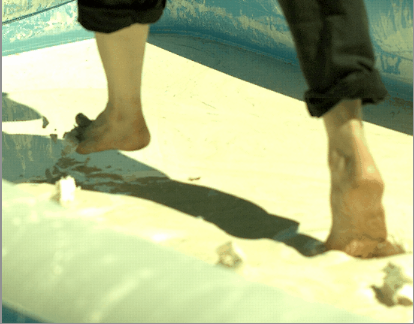
\includegraphics[width=7cm]{image/5-3-1.png}
\caption{在有``弹性''的液体上行走}\label{fig:oobleck}
\end{wrapfigure}
液体在很多方面与气体相似,\,而与固体区分来开.\,具体来说,\,液体没有固定的体积易于流动;\,没有弹性只有黏性;\,黏度与压缩系数比气体倒是大不少,\,这得益于其接近固体的高密度;\,热容,\,热导率等更细节的内容我们后几节详细阐述;\,微观细节则在以后章节中加以说明.\,最后,\,我们指出特殊条件下液体也具有某些与固体相似的性质,\,尤其是当变形率十分的急剧时.\,这种现象是\emph{非牛顿流体}(non-newtonian fluid)的一种典型,\,比如图\ref{fig:oobleck}中用玉米面粉与水和成的\emph{欧不裂}(oobleck)就是一种典型的一旦作用力变化十分快,\,就会主要表现出弹性固体的性质而不是液体的流动性的材料,\,所以人才可以在液面上快步走动而不会陷进去.\,但使我们把液体固体彻底区分开来的主要原因是因为固体具有\emph{序}(order),\,而且是\emph{长程}(long range)的序\footnote{凡事皆有例外,\,\emph{液晶}(liquid crystal)就有长程序的液体,\,\emph{非晶体}(non-crystalline)便是无长程序的固体.\,更准确的液体固体区分方式应该要看结合的强度.}.

\subsection{热容}


\begin{itemize}
	\item 微观结构:\,局部有序,\,有``类晶区''概念,\,\emph{径向分布函数}(radial distribution function)与固体相似.\,但无\emph{长程序}(long range order).\,原子分子时停时动,\,也区别于固体,\,但不像气体那样仅当碰撞时才短暂停驻片刻.
	\item 热容:\,一般来说,\,按原子的摩尔数计算,\,才有等压等体热容约为$3R$
	\item 热膨胀:\,部分液体与晶体反常膨胀,\,结晶过程也不是收缩反而是膨胀,\,一种解释是加热使得一些固体到液体成键倾斜以后更有利于在其他方向节省空间.
	\item 黏度:\,液体一般温度越高黏度越小.\,这是因为不同于气体黏度,\,液体黏度更像固体那样,\,靠的是相互作用形成的``激发''.\,而热运动加剧时液体分子间相互作用更难形成结果,\,比如两个原子很难形成一种亚稳态的``集团''.
\end{itemize}




\section{液体的表面性质}
\begin{itemize}
	\item 液体与气体交界面为\emph{表面}(surface),\,与固体交界面为\emph{界面}(interface).\,表面一般就若干个分子层那么厚,\,表面的分子数密度由于过渡到气体中所以明显会降低.\,界面则可能降低可能升高.
	\item 分子与分子间相互吸引形成内聚力,\,它的计算一般包括在体的内能中.\,但表面与界面的形成会改变能量,\,叫做表面能与界面能.\,它正比于其面积$S$.\,习惯上:
	\[W_s=+\sigma_s S=+\sigma_{\rm lg} S\]
	\[W_i=-\sigma_i S=-(\sigma_{\rm ls}-\sigma_{\rm gs})S\]

	前者$S$为液体表面面积.\,后者$S$为液体固体接触的界面面积,\,就是说要考虑由于液体与固体的接触使得固体与气体少接触了相同的面积可能导致的$\sigma_{\rm gs}S$能量,\,尽管这一项几乎总是可以忽略.\,$\sigma_{\rm ls}$是可正可负可为零的.\,$\sigma_{\rm lg}$一般大于零.

	\item 表面能对应\emph{表面张力}(surface tension):
	\[f_s=\sigma_s L\quad ;\quad f_i=\sigma_i L\]

	前者使表面尽可能小,\,后者使界面尽可能大.

	\item 附加压强的\emph{杨-拉普拉斯方程}(Young-Laplace equation):
	\[\Delta p=\sigma(\frac{1}{\rho_x}+\frac{1}{\rho_y})\]

	其中$\rho_x$和$\rho_y$是可以任意选取的两个相互垂直的方向上曲面上法曲线的曲率.

	\item 液体固体接触的\emph{接触角}(contact angle)的\emph{杨-杜普蕾方程}(Young-Dupr\'e)方程:
	\[\cos\theta=\frac{\sigma_i}{\sigma_s}\]

	若$\sigma_i>0$称为\emph{浸润}(wetting).\,若$\sigma_i>\sigma_s$上式无解称为\emph{完全浸润}(perfect wetting),\,液体会在固体表面尽可能铺展.\,若$\sigma_i\leq 0$称为\emph{不浸润}(non-wetting),\,若$\sigma_i<-\sigma_s$称为\emph{完全不浸润}(perfect non-wetting)

	\item 表面能实际上是自由能而不是内能,\,等温等压拉伸液膜要伴随着吸放热.\,详情参考之前章节的计算.

\end{itemize}



\section{极端条件下的其他物态}

\begin{itemize}
	\item 超冷($\sim {\rm \upmu K}$):\,\emph{玻色-爱因斯坦凝聚}(Bose-Einstein condensate):\,宏观数目的原子的动量$\bs{p}=\hbar \bs{k}$凝聚到了基态.\,其波函数可以被干涉实验探测到.
	\item 低温($1\sim 10{\rm K}$):\,\emph{超流}(superfluid)现象:\,如He-4液体黏度消失.\,He-3由于是费米子其超流直到1970年代才被发现,\,需要$\sim {\rm mK}$的低温.
	\item 低温物理中的高温($10\sim 100{\rm K}$):\,\emph{超导}(superconductor):\;常规金属的电阻率会消失,\,伴随着\emph{迈斯纳效应}(Meissner effect):\,完全抗磁性.\,电子结合成\emph{库珀对}(Cooper pair),\,可以像BEC那样通过晶格作用而凝聚成整个波函数而传播.

	\item 高温低密($10^3 \sim 10^4{\rm K}$):\,\emph{等离子体}(plasma),\,所有电子都与原子核不再形成束缚态,\,而是构成独立的气体体系,\,可以不考虑相对论效应也不考虑电子的量子简并来处理.\,

	\item 超高温,\,高密度($10^{11} \sim 10^{12}{\rm K},\,10^{17}{\rm kg/m^3}$):\,引力场下坍缩形成的中子星.\,电子数不再守恒而是在中子质子互变的反应中产生与消灭.\,

	\item 最高温($>10^{12}{\rm K}$):\,各大型对撞机上已经实现的\emph{夸克-胶子等离子体}(quark-gluon plasma):\,质子数和中子数不再守恒,\,内部的构成的夸克与胶子形成强相互作用的等离子体.\,

	\item 每一种粒子数不再守恒的极端相对论性的气体,\,其内能密度与温度的关系都是:\,对于每自由度的玻色子与费米子:
	\[u_b=\frac{2\sigma}{c}T^4\quad ;\quad u_f=\frac{7}{8}u_b\]

	例如对于光子气,\,两个偏振自由度再结合$J=uc/4$便得到黑体辐射公式.\,对于不包含第二代基本粒子的QGP,\,夸克有2味3色2自旋2电荷一共24自由度,\,胶子有8色2偏振(螺度)共16自由度.\,代入得:
	\[u=\frac{74\sigma T^4}{c}\]
\end{itemize}